\documentclass{amsart}
\usepackage{graphicx}

\begin{document}
\author{ Catherine Zuo, Kimberly Toy,and Will Oursler}
\title{Design Notes}
\date{\today}
\maketitle

This document contains rough design guidelines. These guidelines should be carefully fleshed out and discussed, both before coding, and during coding as problems become apparent.

\section{ Dependency Graph }

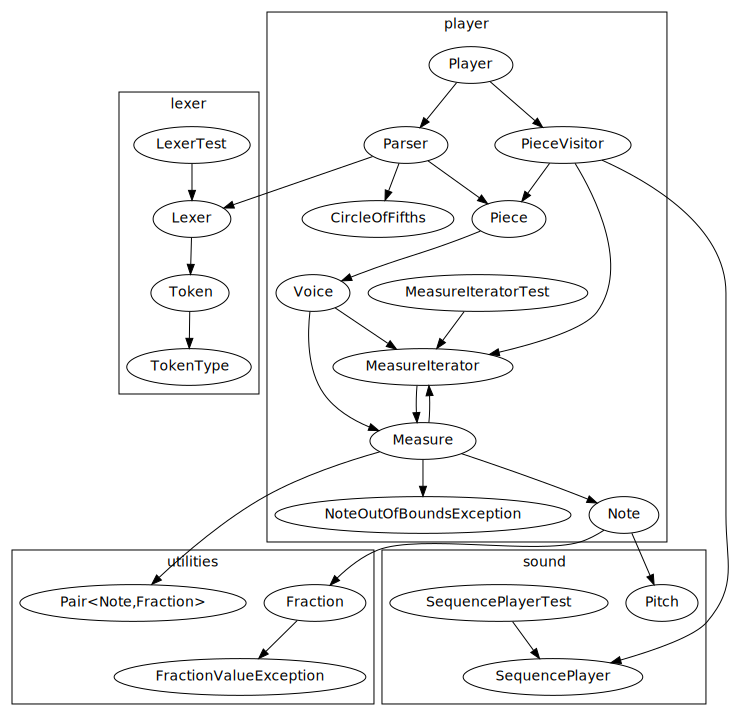
\includegraphics[width=\linewidth]{classes.png}

\section{ The Fraction class }

Because note lengths and start times are all rational numbers, and because the exact ratios of these numbers with respect to others is important, a Fraction method is useful.

The Fraction class has a Numerator and Denominator, guaranteed to be in lowest terms. It supports addition and multiplication ( possibly division and subtraction if w have time ).  In order to add and multiply while keeping the Fraction in simplest terms, we also implemented GCD and LCM methods.  

\section{ The Piece class }

This class is primarily concerned with the piece metadata, such as BPM, time, etc. It also contains a reference to the first Measure of the piece.  It is a mutable class and has methods to set the piece's voices.  

\section{ The Measure class and Repeats }

Each measure is a container of Note instances, each Note being associated with a start time ( represented by a Fraction ) relative the beginning of the measure. In this manner, the same Measure object can represent both of its instantiations in a repeat. Measures are structured similarly to a linked list, but have an additional pointer to a second next element. If the Visitor has seen a specific measure before (measured by reference NOT value, as two different measures may contain the same musical content), it will take the second next measure rather than the first. This perhaps should be enabled with a careful Iterator pattern, using a MeasureIterator class.  

Measures are mutable objects and contain methods to changing the measure's pointers to other measures and adding or modifying what notes are in the method.  

MeasureIterator is an Iterator which helps the Visitor accurately navigate through the 'linked list' of Measures.  

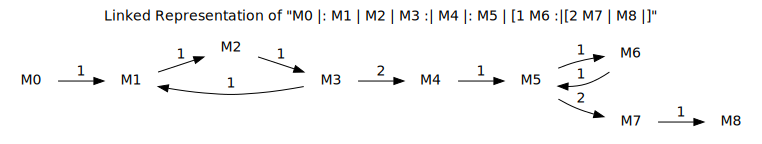
\includegraphics[width=\linewidth]{measure_example.png}

\section{ The Note class }
A Note contains a pitch and a duration  ( represented by a Fraction ).  It does NOT contain any information that refers to a larger data structure. The key signature / implicit accidentals, for instance, are not relevant. They should be handled by the Parser.

Rests are not notes, and in fact are not represented at all; they are redundant because note start times are explicitly specified by the Parser.

Notes are immutable objects.  Its values are pitch, length, accidentals, octave, and it has getter methods to access these values.  

\section{ Lexer }
The Lexer class will separate the input into tokens.  For the header of the piece, it will create field header tokens, field value tokens, and newline tokens to show the separation between fields and the header and body.  
For the body of the piece, it will create tokens for note pitches, which includes an upper or lowercase letter, accidental, or octave ticks, note length values, chords, tuplets, rests, bar lines, and the symbols indicating that there are multiple voices.  It will also ignore whitespace and comments.
The lexer will throw exceptions when it encounters invalid symbols or malformed tokens.  

\section{ Parser }
The parser will parse the header information tokens, specifically identifying key signature (using Circle of Fifths class), the tempo, and the time signature.  It will throw errors if there are invalid (or null) values for any of these fields.  This information will be passed into the Piece data type.  

The parser will parse the body tokens into Measures, with methods to create note objects from single notes, tuples, chords, and rest Tokens.  From the key signature, the parser should keep track of current accidentals throughout a Measure, resetting when creating a new Measure.  The parser must link the next measure to the previous measure (e.g. the case of multiple endings).  In addition, it should keep track of different beat divisions, which will be used by the Visitor to determine a common tick/measure for the entire Piece.  Also, it should note if there are multiple voices and create separate 'linked lists' of Measures for each voice if so.  

Some errors that parser will keep an eye out for: invalid measure durations (too long or too short), incorrect repeat braces, musically incorrect accidental stacking, invalid tuplets (length-wise), and invalid beat times (negatives, decimals, and the Fraction class should ensure there are no divide by 0s). 

\section{ Visitor }
The Visitor interfaces with the Piece class and the SequencePlayer.  It tracks global time as it goes through the Piece's linked list(s) of Measures, using MeasureIterator.  From the information about the different beat divisions it calculates the number of ticks/quarter note (using LCM of all beat divisions).  Thus, when it goes through a Measure and transcribes the notes to MIDI format, it correctly translates the note's local time to a global time.  When visiting measures, it will follow the measure's first pointer to another measure, if the measure has never been visited.  Otherwise, it will visit the second pointer.  (There is a possible bug here - in the case of nested repeats, it could possibly follow the first pointer in an infinite loop - a possible solution is using a stack of hash maps).  In addition, it should accurately handle multiple voices.  

\section{ Testing }
The modularity of our design allows that each major class can be tested.  We test that...

... the Lexer can separate every kind of token, throws exception of invalid tokens, and correctly handles null input.

... the Parser throws exceptions for all errors; correctly parses Measures with both basic notes and more complex tokens (chords, tuples); correctly creates nested repeat structures and multiple endings.  

... the Visitor ensures global timekeeping is working and correctly translates to MIDI notes; correctly calculates a 'base' tick/quarter note from the different beat divisions; correctly traverses through repeats and alternate endings; and ensures that errors thrown in Lexer/Parser also stop its actions.   

\end{document}
